\section{成员函数与友元函数}
在上一节中,我们讲了一些非成员函数形式的运算符重载,并见识到了它的方便之处。不过使用非成员函数也存在一些缺点,比如说:
\begin{itemize}
    \item 非成员函数不属于这个类,所以不能访问这个类的私有成员。如果要进行什么操作,我们只能走曲线,通过那个类的成员函数来访问它。这样的确很有安全性,但其麻烦也是显而易见的。
    \item 一些运算符只能定义为成员函数,不能作为非成员函数存在,比如下标运算符。
\end{itemize}
很容易想到的解决方法当然是——把我们想要重载的运算符定义为成员函数。\par
我们就以 \lstinline@std::valarray@ 为例吧。它是一个类模版,和 \lstinline@std::vector@ 一样近似于数组。它们的区别在于,\lstinline@std::vector@ 更关注数据的存储和动态操作,而对计算性质的支持较少;而 \lstinline@std::valarray@ 则在数据的批量计算方面支持了更丰富的功能,但在数据存储和动态操作方面几乎没有什么功能。下面的例子展示了 \lstinline@std::valarray@ 在批量计算方面的效果,这是原生 \lstinline@std::vector@ 无法做到的。
\begin{lstlisting}
//需要包含valarray库
    std::valarray<double> arr {-2.57,-0.987,0.57,2.14159};
    std::valarray<double> arr1 {arr + 1}; //每个数都增加1
    std::valarray<double> arr2 {std::sin(arr)}; //直接求出每个数的正弦值
    for (int i = 0; i < arr1.size(); i++) {
        std::cout << arr1[i] << ' '; //输出arr1的每个数,以供验证
    }
    std::cout << std::endl;
    for (int i = 0; i < arr2.size(); i++) {
        std::cout << arr2[i] << ' '; //输出arr2的每个数,以供验证
    }
    std::cout << std::endl << arr2.sum(); //sum()成员函数返回arr2所有数的和
\end{lstlisting}
这段代码的运行结果如下:\\\noindent\rule{\linewidth}{.2pt}\texttt{
-1.57 0.013 1.57 3.14159\\
-0.540972 -0.834376 0.539632 0.841472\\
0.0057561
}\\\noindent\rule{\linewidth}{.2pt}
看起来运行结果十分符合预期。这也就是 \lstinline@valarray@ 的强大之处。\par
\lstinline@std::valarray@ 看起来十分好用。我们也可以自行定义一个 \lstinline@valarri@ 类,并配备这些功能。
\begin{lstlisting}
#include <initializer_list>
class valarri {
public:
    valarri(const std::initializer_list<int> &initl) { //留到下一节再讲
        _size = 0;
        for (int x : initl)
            _arr[_size++] = x;
    }
    //...
private:
    static const std::size_t MAX_SIZE {100};
    int _arr[MAX_SIZE];
    std::size_t _size;
};
\end{lstlisting}
其中的 \lstinline@valarri@ 成员是一个构造函数,我们会在下一节中介绍构造函数相关的知识。这里读者不必纠结,直接把它抄进 \lstinline@valarri@ 类的定义中就可以了。\par
接下来我们就看一下,有哪些我们需要的成员函数。\par
\subsection*{成员函数的声明与定义}
首先我们需要一个 \lstinline@size@ 成员函数,它是公有的,能让外界知道这个数组存了多少数据。
\begin{lstlisting}
public:
    std::size_t size() { //返回值是数组当前的存储量
        return _size; //返回私有成员_size
    }
\end{lstlisting}\par
原生的 \lstinline@std::valarray@ 不支持 \lstinline@push_back@, \lstinline@pop_back@ 等操作,所以我们可以不管。\par
为了方便地返回这个数组中的最大值,最小值和总和,我们可以定义 \lstinline@max@, \lstinline@min@ 和 \lstinline@sum@ 成员函数。这里的 \lstinline@max@ 和 \lstinline@min@ 不会与 \lstinline@std::max@ 和 \lstinline@std::min@ 冲突,不仅是因为它们属于不同的命名空间,还因为它们之间有着``成员''与``非成员''的区别。读者会在实际编程中慢慢领悟到这一点的。
\begin{lstlisting}
public:
    int max() { //返回值是数组当前的最大值
        int maximum {_arr[0]}; //先假设arr[0]就是最大值
        for (int i = 1; i < _size; i++)
            if (maximum < _arr[i]) //一旦遇到了一个比maximum更大的
                maximum = _arr[i]; //就把maximum变成这个数
        return maximum;
    }
    int min() { //返回值是数组当前的最小值
        int minimum {_arr[0]}; //先假设arr[0]就是最小值
        for (int i = 1; i < _size; i++)
            if (minimum > _arr[i]) //一旦遇到了一个比minimum更小的
                minimum = _arr[i]; //就把minimum变成这个数
        return minimum;
    }
    int sum() { //返回值是当前数组中有效数据的总和
        int summation {0}; //先置为0
        for (int i = 0; i < _size; i++)
            summation += _arr[i]; //然后把每个数都加到summation上
        return summation;
    }
\end{lstlisting}
然后我们只需要把这些内容都整理到 \lstinline@valarri@ 的定义中就行了。\par
但是当我们真的把一大堆成员函数的定义都写在类定义中的时候,我们就会发现这些内容非常冗长,即便我们把排版做得再好,也还是会有重点不突出的感觉。回想一下我们在7.1节中讲过的例子,那时我们在一个头文件中声明函数,在一个源文件中定义函数,而又在另一个源文件的主函数中调用这些函数。这种结构多么清晰,多么一目了然啊。\par
在定义成员函数的时候,我们也可以把声明和定义分开写,成员声明写在类的定义内部,而成员定义写在类的定义外部。所以我们可以把这个类的定义写成这样:
\begin{lstlisting}[caption=\texttt{Header.h}]
//头文件部分
#pragma once
#include <initializer_list>
class valarri {
public:
    valarri(const std::initializer_list<int>&); //声明构造函数
    std::size_t size() { return _size; } //这个函数很短,一行就够,直接定义吧
    int max();
    int min();
    int sum(); //声明max, min和sum
    //...待补充
private:
    static const std::size_t MAX_SIZE{ 100 };
    int _arr[MAX_SIZE];
    std::size_t _size;
}; //这样就整洁多了吧
\end{lstlisting}
这个部分的内容可以放到头文件中。\par
接下来我们在类的外部进行定义,可以把它放到某个源文件中。不过我们不要忘了,我们是在类作用域的外部进行定义,如果我们直接写成
\begin{lstlisting}
int max() {/*...*/} //这是在定义::max
\end{lstlisting}
这样编译器就会把它当作是一个非成员函数来看待,这不是我们想要的。为了区分,我们需要用作用域解析运算符来指明:我们是在定义 \lstinline@valarri@ 类的 \lstinline@max@ 成员函数。
\begin{lstlisting}[caption=\texttt{Definition.cpp}]
//源文件部分
#include "Header.h"
int valarri::max() { 我们定义的函数是valarri::max,不是::max;而返回类型是int
        int maximum {_arr[0]};
    for (int i = 1; i < _size; i++)
        if (maximum < _arr[i])
            maximum = _arr[i];
    return maximum;
}
int valarri::min() {
    int minimum {_arr[0]};
    for (int i = 1; i < _size; i++)
        if (minimum > _arr[i])
            minimum = _arr[i];
    return minimum;
}
int valarri::sum() {
    int summation {0};
    for (int i = 0; i < _size; i++)
        summation += _arr[i];
    return summation;
}
valarri::valarri(const std::initializer_list<int> &initl) {
    _size = 0;
    for (int x : initl) {
        _arr[_size] = x;
        ++_size;
    }
} //定义的顺序无所谓,不用非得按照声明的顺序来
\end{lstlisting}
这些就是声明的部分,我们可以把它放到一个源文件中,然后就可以在另一个源文件中调用它们了。\par
\subsection*{成员形式的运算符重载}
非成员形式的运算符重载有比较多的限制,所以我们就来看看成员形式的运算符重载。\par
这两种运算符重载没有本质上的不同,它们接收参数的个数都是一样的,它们的优先级、结合性也是一样的。但在语法上,它们还是有区别的。\par
\subsubsection*{加法运算符的重载}
举个例子,如果我们要重载加法运算符,以支持两个 \lstinline@valarri@ 类对象直接相加,我们应该这样声明和定义:
\begin{lstlisting}
//声明部分
public:
    valarri operator+(const valarri&); //重载加法运算符,以进行两数组加法
    valarri operator+(int); //重载加法运算符,以进行数组与数的加法
//定义部分,记得#include<algorithm>,因为这里用到std::min了
valarri valarri::operator+(const valarri &a) { //重载valarri成员函数operator+
    valarri v {}; //这里好像不能省略花括号?我们到了下一节再讲它
    v._size = std::min(_size, a._size); //这里有三个_size成员,需要区分开
    for (int i = 0; i < v._size; i++)
        v._arr[i] = _arr[i] + a._arr[i]; //这里也有三个_arr成员,需要区分开
    return v; //返回值是v
}
valarri valarri::operator+(int n) { //重载valarri成员函数operator+
    valarri v {}; //同样不能省略花括号
    v._size = _size; //这两个_size成员不是同一个东西
    for (int i = 0; i < v._size; i++)
        v._arr[i] = _arr[i] + n; //这两个_arr成员不是同一个东西
    return v; //返回值是v
}
\end{lstlisting}
读者可能关心以下几个问题,我将逐一说明:\par
{\kaishu 为什么重载的加法运算符只接收了一个参数?不是说,成员函数接收的操作数个数不变吗?}\par
我们在下一节中会讲到,任何一个成员函数都带有一个隐藏参数,即``调用此函数的对象''。以 \lstinline@size@ 成员函数为例,当我们调用它的时候,比如写成 \lstinline@_arr.size()@。这里看似不需要传递参数;但在汇编代码中我们就可以看出,实际上这个过程把 \lstinline@_arr@ 以指针(或引用)的形式传递过去了。\par
对于运算符来说也同理。这里的 \lstinline@valarri+(const valarri &a)@ 还有一个隐藏参数,就是调用它\footnote{成员运算符也可以用成员访问的形式来调用,比如 \lstinline@arr1+arr2@ 也可以写成 \lstinline@arr1.operator+(arr2)@。但是这样调用就比较麻烦了,还不如自己写个函数。}的对象本身;另一个参数是这里的 \lstinline@a@。
\begin{lstlisting}
    valarri arr1 {}, arr2 {};
    arr1 = arr1 + arr2; //arr1调用了这个函数,arr2就是形参a对应的实参
\end{lstlisting}\par
{\kaishu 为什么我们有的时候用 \lstinline@_arr@,有的时候用 \lstinline@v._arr@ 和 \lstinline@a._arr@ 呢?它们分别代表什么?}\par
我们在用某个对象来调用成员函数时,只能把这个对象以``匿名''的方式作为参数传递——比如说吧,\lstinline@arr1@ 调用加法运算符时虽然也作为参数传入,但是它对应的形参是什么?我们不知道它的名字。这就会造成一个问题:如果我们想要访问它的成员,那该怎么办?\par
常规的解决方法有两种。第一种最直观,那就是压根不需要用成员访问运算符,直接写成 \lstinline@_arr@ 和 \lstinline@_size@;第二种我们稍后再讲。以这句代码为例:
\begin{lstlisting}
    v._size = std::min(_size, a._size);
\end{lstlisting}
它有三个 \lstinline@_size@ 成员出现。\lstinline@v._size@ 和 \lstinline@a._size@ 分别是 \lstinline@v@ 和 \lstinline@a@ 的成员,这个不会搞混吧。而 \lstinline@_size@ 正是``调用此运算符的对象''的成员。\par
如果放在 \lstinline@arr1+arr2@ 的情境下,那么 \lstinline@_size@, \lstinline@a._size@ 和 \lstinline@v._size@ 分别对应 \lstinline@arr1._size@\footnote{这只是象怔性的写法,实际上 \lstinline@arr1._size@ 的写法相当于在 \lstinline@valarri@ 的类作用域外部访问该类的私有成员,这是禁止的。}, \lstinline@arr2._size@ 和 \lstinline@(arr1+arr2)._size@\footnote{初学者可能对 \lstinline@(arr1+arr2)._size@ 这种写法感到困惑,但是不要忘记,\lstinline@arr1+arr2@ 的返回值也是一个 \lstinline@valarri@ 类型的对象,所以它当然也有自己的成员咯。}。图8.1展示了它们之间的关系。\par
\begin{figure}[htbp]
    \centering
    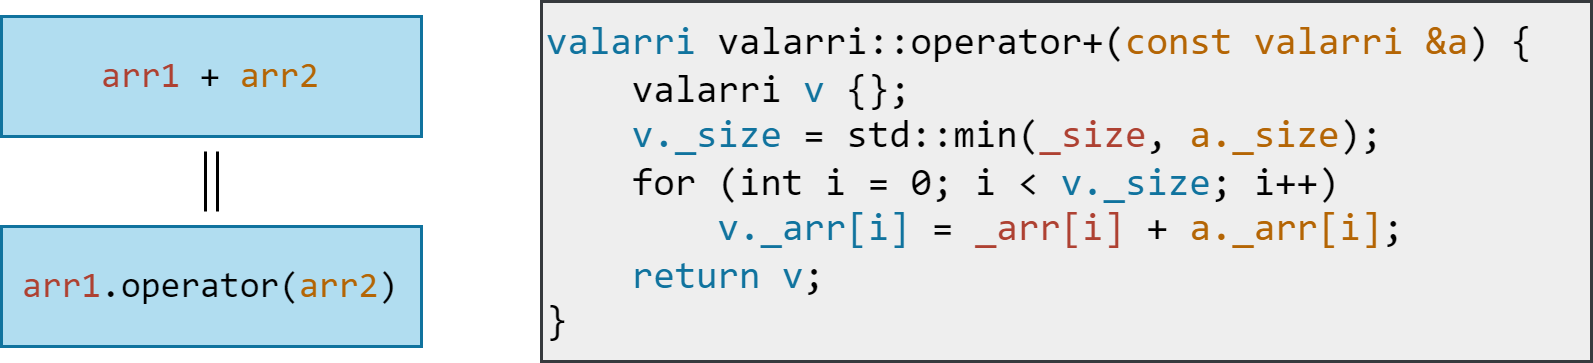
\includegraphics[width=\textwidth]{../images/generalized_parts/08_operator_overloading_as_member_function_300.png}
    \caption{\lstinline@arr1+arr2@ 调用过程中的三个对象及其成员}
    \footnotesize{以红色、橙色、蓝色区分这三个对象的相关信息}
\end{figure}
其它的算术运算符,比如四则运算和位运算,也可以仿照此法进行重载,这里就不再赘述了。\par
\subsubsection*{下标运算符的重载}
下标运算符的重载很简单,直接写就行了。
\begin{lstlisting}
//函数定义很短,所以直接定义也行
public:
    int& operator[](int i) { //如果允许通过下标运算符改变数组的值,那就用int&
        return _arr[i];
    }
\end{lstlisting}
这里的返回类型是 \lstinline@int&@,所以如果我们修改下标运算符的返回值,那么我们也就直接修改了数组当中的内容。\par
下标运算符的返回值并不局限于整型,或者可以隐式转换为整型的类型。任何类型都可以作为下标存在。举个例子来说,\lstinline@std::map@ 是定义在头文件 \lstinline@map@ 当中的类模版,它表示的是一种映射关系。对于 \lstinline@std::map<Key,T>@ 来说,我们可以用 \lstinline@Key@ 类的键(或者说,索引)数据来找到对应的 \lstinline@T@ 类数据。\lstinline@std::map@ 重载了下标运算符 \lstinline@[]@:
\begin{lstlisting}
T& operator[](const Key &key);
T& operator[](Key &&key);
\end{lstlisting}
这样一来,我们就可以通过下标运算符,方便简单地使用 \lstinline@Key@ 类的数据找到 \lstinline@T@ 类的值。\par
\subsubsection*{\texttt{this}指针与赋值运算符的重载}
C++内置类型的变量都支持赋值\footnote{常量和常量表达式不能赋值。所以这里所指的变量不包含常量。},这是改变一个数值的最简单、最直接、最常用的方式——难怪高德纳会把赋值语句和指针变量共同视作计算机科学中最有价值的宝藏。那么我们能不能重载赋值运算符,以此实现 \lstinline@valarri@ 类对象间的直接赋值呢?答案当然是肯定的。\par
赋值运算符的返回值是对左操作数的引用,所以在这里,我们也需要返回一个对左操作数的引用。但是当我们真的写起这个函数时就会发现情况好像不太对:
\begin{lstlisting}
//声明部分
public:
    valarri& operator=(const valarri&);
//定义部分
valarri& valarri::operator=(const valarri&){
    //在这里实现赋值的主要部分
    return /*等下,这里要返回什么?*/;
}
\end{lstlisting}
在这里我们遇到了困难。左操作数是作为匿名形参传入的,我们要怎么表达``调用这个函数的对象''呢?如果表达不了的话,那我们岂不是就无法返回这个对象了吗?在这种情形下,我们就必须要用 \lstinline@this@ 了。\par
\lstinline@this@ 是一个关键字,它代表的含义是一个指针。不过 \lstinline@this@ 不是传统意义上的指针,它只能在非静态成员函数等地方出现。它只能表示一个地址值,不能被修改(像是常量指针);但我们可以通过这个地址值取内容,进而修改它指向的对象——它指向的对象正是``调用此函数的对象''。\par
既然它指向的就是``调用此函数的对象'',那么我们以 \lstinline@*this@ 作为返回值不就好了?\par
另外,因为 \lstinline@this@ 指向的就是``调用此函数的对象'',那么我们用指针的成员访问运算符,岂不是也可以解决前文中提到的问题?
\begin{lstlisting}
        v._arr[i] = this->_arr[i] + a._arr[i];
\end{lstlisting}
当然了,这种写法还是比较麻烦。所以倘若没有消歧义的需要,我们就不必这样写,直接用 \lstinline@_arr[i]@ 就可以了。\par
回到赋值运算符的重载。对于赋值运算符来说,我们需要防范一种特殊情况,就是自我赋值。
\begin{lstlisting}
    arr1 = arr1; //这是需要特殊考虑的!
\end{lstlisting}
如果进行了自我赋值,那就应该什么也不做直接返回 \lstinline@*this@,否则就是在浪费时间。
\begin{lstlisting}
valarri& valarri::operator=(const valarri &a) { //其中的a应作为常量引用
    if (&a == this) //检测a的地址是否与本对象一致
        return *this; //如果一致,直接返回*this
    //...
}
\end{lstlisting}\par
排除了这个特殊情况之后,我们就可以处理一般情况了,也很简单。
\begin{lstlisting}
valarri& valarri::operator=(const valarri &a) { //返回类型和参数均为引用
    if (&a == this) //检测a的地址是否与本对象一致
        return *this; //如果一致,直接返回*this
    _size = a._size; //记得更改_size
    for (int i = 0; i < _size; i++)
        _arr[i] = a._arr[i]; //有效数据范围内的每个数都要赋值,后面的可以不管
    return *this; //返回*this
}
\end{lstlisting}\par
我们还可以重载复合赋值运算符,就以加赋值运算符 \lstinline@+=@ 为例吧。在这里我们也进行了代码重用,从而让我们写起函数更简单。
\begin{lstlisting}
//声明部分
public:
    valarri& operator+=(const valarri&); //重载加赋值运算符,可以加之以数组
    valarri& operator+=(int); //重载加赋值运算符,可以加之以数
//定义部分
valarri& valarri::operator+=(const valarri &a) {
    return *this = *this + a; //利用已经重载的赋值运算符和加法运算符
}
valarri& valarri::operator+=(int n) {
    return *this = *this + n; //利用已经重载的赋值运算符和加法运算符
}
\end{lstlisting}\par
\subsection*{友元函数}
在重载加法运算符时,我们只有``数组+单个数字''的版本:
\begin{lstlisting}
valarri valarri::operator+(int n);
\end{lstlisting}
不过,加法运算满足交换律,所以我们也应当有一个``单个数字+数组''的版本。但是当我们真的要实施起来的时候,就会发现困难所在:\par
我们不能把这个运算符重载为成员函数,因为成员函数的第一个参数必须是 \lstinline@valarri@ 类型,但我们期望它是 \lstinline@int@ 类型。\par
但是当我们试图重载一个非成员函数时,我们又会遇到新的麻烦:
\begin{lstlisting}
valarri operator+(int n, const valarri &a) {
    valarri v {};
    v._size = a._size;
    //error: 'std::size_t valarri::_size' is private within this context
    for (int i = 0; i < v._size; i++)
    v._arr[i] = a._arr[i] + n;
    //error: 'int valarri::_arr [100]' is private within this context
    return v;
}
\end{lstlisting}
编译器的报错信息含义很明显,我们不能通过非成员函数访问私有成员 \lstinline@_size@ 和 \lstinline@_arr@。\par
这里我们有很多解决方法,比如说直接在函数中返回 \lstinline@a+n@。
\begin{lstlisting}
valarri operator+(int n,const valarri &a) {
    return a+n; //代码重用
}
\end{lstlisting}\par
但我们还是需要一种方法,让我们可以在特定条件下,从外界访问某个类的私有成员。我们的答案是友元\footnote{以笔者的观点看,友元(Friend)这个名字实在容易让人误会。友元是一种单向关系不是双向关系,但friend几乎都是表示双向关系的。对于友元函数来说单向双向无所谓,但是对于友元类来说是有所谓的。}。\par
声明一个友元函数的方法很简单,就是在类当中,用 \lstinline@friend@ 关键字加这个函数,以此表示``该函数可以访问此类的私有/受保护对象''。
\begin{lstlisting}
//友元声明部分
class valarri {
    //...
    friend valarri operator+(int, const valarri&);
    //声明此函数为valarri的友元函数
};
//定义部分
valarri operator+(int n, const valarri &a) { //定义valarri的友元函数operator+
    valarri v {};
    v._size = a._size;
    for (int i = 0; i < v._size; i++)
        v._arr[i] = a._arr[i] + n;
    return v;
} //一切顺利
\end{lstlisting}\par
我们还可以把友元声明和定义放到一起。
\begin{lstlisting}
class valarri {
    //...
    friend valarri operator-(int n, const valarri &a) { //定义减法友元
        valarri v {};
        v._size = a._size;
        for (int i = 0; i < v._size; i++)
            v._arr[i] = n - a._arr[i];
        return v;
    }
};
\end{lstlisting}
但是请读者注意,\textbf{即便友元函数的定义写在 \lstinline@class@ 内部,它也是非成员函数}(如果是成员函数的话那就没必要友元了嘛),因此参数列表必须写两个形参(而不是一个形参加一个不具名参数),而且函数体中不能使用 \lstinline@this@。\par
\subsubsection*{友元是二者的关系,而非一者的性质}
还有一个常见的例子是输入。我们可以用 \lstinline@std::istream@ 类的对象 \lstinline@cin@ 来为一个 \lstinline@int@ 型变量或者 \lstinline@double@ 型变量输入其值,但是我们不能直接输入一个 \lstinline@valarri@ 类的对象。有的时候我们会有这方面的需要,所以我们需要写一个运算符,能够直接实现 \lstinline@std::cin>>a@。\par
让我们考虑一下——要实现这个目的的主要困难在于,其一,我们不能修改标准库代码\footnote{任何时候都不要修改标准库中的代码。——笔者的忠告},所以我们肯定不能把这个功能写成 \lstinline@std::istream@ 的成员函数;其二,因为左操作数是 \lstinline@std::cin@,不是 \lstinline@valarri@ 类,所以我们也不能把这个功能写成 \lstinline@valarri@ 的成员函数。\par
所以我们只剩下一条路,那就是非成员函数。这里我们必须要修改 \lstinline@valarri@ 的私有成员,所以我们需要把它定义成 \lstinline@valari@ 的友元函数。
\begin{lstlisting}
//友元声明部分
class valarri {
    //...
    friend std::istream& operator>>(std::istream&, valarri&);
    //需要包含iostream头文件
};
//定义部分
std::istream& operator>>(std::istream& in, valarri& a) {
    a._size = 0; //因为它是valarri的友元,所以可以访问valarri的私有成员
    while (in && a._size < a.MAX_SIZE) //要保证in正常且a._size不达到最大容量
        in >> a._arr[a._size++]; //注意++是后置的,不是前置
    if (!in) //检测一下in的状态,保证其状态正常
        input_clear(in); //这次就不是用默认参数,而是用in了
    return in; //返回in,以便连续赋值
}
\end{lstlisting}
需要提醒读者,这个运算符只是 \lstinline@valarri@ 的友元,它不是 \lstinline@std::istream@ 的友元——我们并没有在 \lstinline@std::istream@ 的定义当中声明这个友元。在这里,我们也不需要它是 \lstinline@std::istream@ 的友元,因为我们并没有使用这个类的什么私有成员,我们只用它的公有成员来完成这些操作。\par
总之,\textbf{友元并不是某个函数或某个类的性质,它是函数与类、类与类之间的关系}。而且这种关系是单向的:A是B的友元,并不意味着B是A的友元。\par
